\documentclass{beamer}

\usepackage[utf8x]{inputenc} %arregla tema tildes y ñ
\usepackage[activeacute,spanish]{babel}
\usepackage{tikz}
\usepackage{wrapfig} % para meter fotitos volando por ahí
\usepackage{graphicx}
\usepackage{subfigure}

\usetikzlibrary{arrows,shapes,arrows,chains,matrix}
%\usepackage[pdftex]{color}

%Tema
\usetheme{Warsaw}
%\usetheme{Berlin}


%\tikzstyle{blockPeque} = [rectangle, draw, thick,draw=gray!80,fill=gray!20,
%text width=80px, text centered, rounded corners, minimum height=13px,node distance = 3cm]

%Portada
\title{RF$^{2}$ - Recarga Fácil por Radio Frecuencia}
\author{Daniel Aicardi, Melina Rabinovich, Edgardo Vaz} 
\institute{
	Tutores: Ing. Juan Pablo Oliver, Ing. Andrés Aguirre\\

\bigskip
\bigskip
	Facultad de Ingeniería - UdelaR\\
	
	\bigskip
	
\includegraphics[scale=.2]{Imagenes/logos.jpg} \\%remove this line if no logo.
}

\date{\today}

\begin{document}

%Portada
\begin{frame}[plain]
	\titlepage
\end{frame} 


\begin{frame}\frametitle{Esquema de la presentación}
	\scriptsize 
	\tableofcontents
\end{frame}


%esto es para ejemplo nomás
\section{Introducción}

\subsection{Sistema de Transporte}
\begin{frame}

%	\begin{wrapfigure}{r}{.5cm}
%		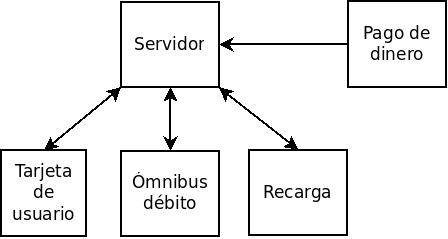
\includegraphics[scale=.5]{Imagenes/sistrans.jpg}
%	\end{wrapfigure}

	\begin{itemize}
		\item el pasajero usa su tarjeta como método de pago
		\item dispositivo lector a bordo que debita viajes
		\item recargar tarjetas
		\item sistema de gestión de negocios (servidores, seguridad, puntos de venta)
	\end{itemize}
\end{frame}

\begin{frame}
	\frametitle{Recarga hoy}
	
	Al día de hoy:
	\begin{itemize}
		\item mundo PC
		\item puntos de venta concentrados
		\item pago no desacoplado de la recarga
		\item no está pensado 24/7		
	\end{itemize}
\end{frame}

\begin{frame}
	\frametitle{Solución alternativa}
	
	Alternativa:
	\begin{itemize}
		\item mundo sistemas embebidos
		\item puntos de venta bien distribuídos
		\item pago desacoplado de la recarga
		\item 24/7		
	\end{itemize}
\end{frame}

\subsection{Proyecto RF$^{2}$}
\begin{frame}
	\frametitle{Objetivos}
		\begin{block}{Objetivo principal}		
			Diseño y fabricación de un prototipo para recargar y consultar tarjetas RFID
		\end{block}
		
		Características principales del prototipo:
		\begin{itemize}			
			\item autónomo
			\item seguro
			\item bajo costo
			\item bajo consumo
			\item bajo mantenimiento
		\end{itemize}

\end{frame}

\begin{frame}
	\frametitle{Descripción del prototipo}
	\begin{itemize}
		\item sistema basado en un microprocesador (SBC)
		\item lector/escritor de tarjetas RFID (antena)
		\item lector/escritor de tarjetas de contacto (SAM)
		\item interfaz de usuario
	\end{itemize}
\end{frame}

\begin{frame}
	\frametitle{Antecedentes}
	\begin{itemize}
		\item existen antecedentes de todas las partes
		\item lectores/escritores de tarjetas RFID y de contacto orientados a PC 
		\item OpenPCD - hardware y software abierto
		\item AFE - dispositivo autónomo hecho en IM
	\end{itemize}	
\end{frame}

\begin{frame}
	\frametitle{Elección de arquitecturas}
	\begin{itemize}
		\item varias alternativas, muchas similares entre sí
		\item 2 más factibles
	\end{itemize}
	\textcolor{red}{acá van imágenes de las 2 arq!!!}
	
\end{frame}

\begin{frame}
	\frametitle{Arquitectura, con OpenPCD vs. prototipo RF$^{2}$}
	\begin{center}
		\scalebox{0.8}{
		\begin{tabular}{c|c}
			OpenPCD & RF$^{2}$ \\ \hline
			dispara los costos & costos razonables\\
			dispositivo orientado a PC & dispositivo autónomo\\
			arquitectura similar al AFE & -\\
			- & diseño del lector/escritor RFID desde cero!!
		\end{tabular}}	
	\end{center}
\end{frame}

\begin{frame}
	\frametitle{Arquitectura definida}
	\begin{center}
		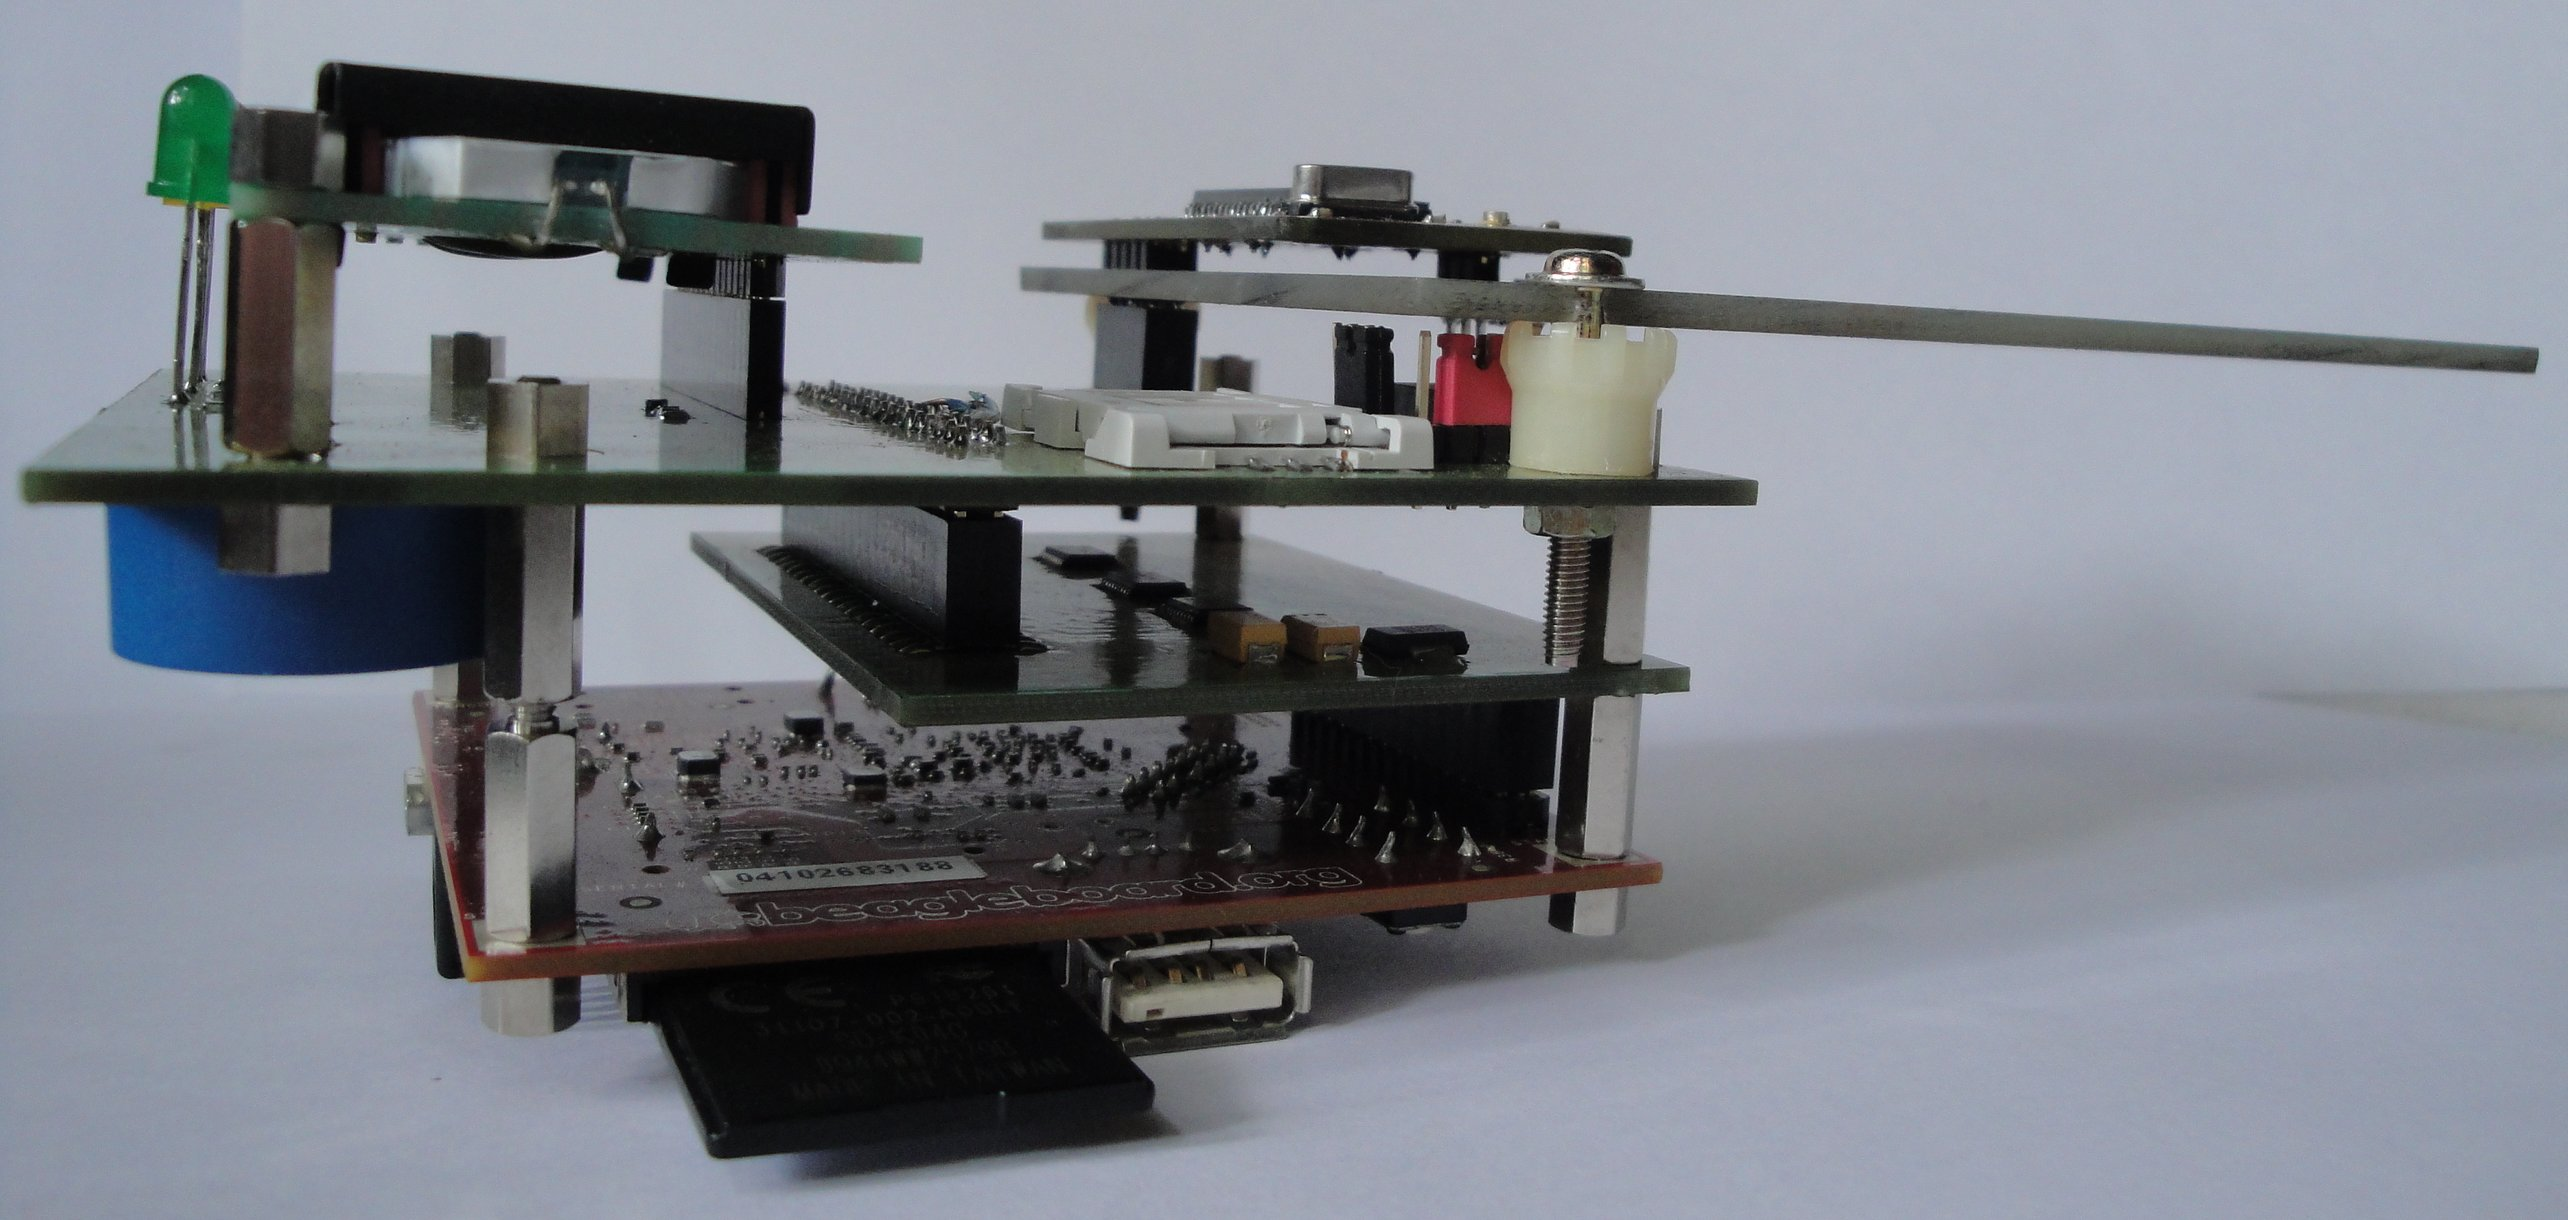
\includegraphics[scale=.12]{Imagenes/prototipo_s.jpg}
	\end{center}
\end{frame}


\begin{frame}
	\frametitle{Arquitectura definida}
	\begin{center}
		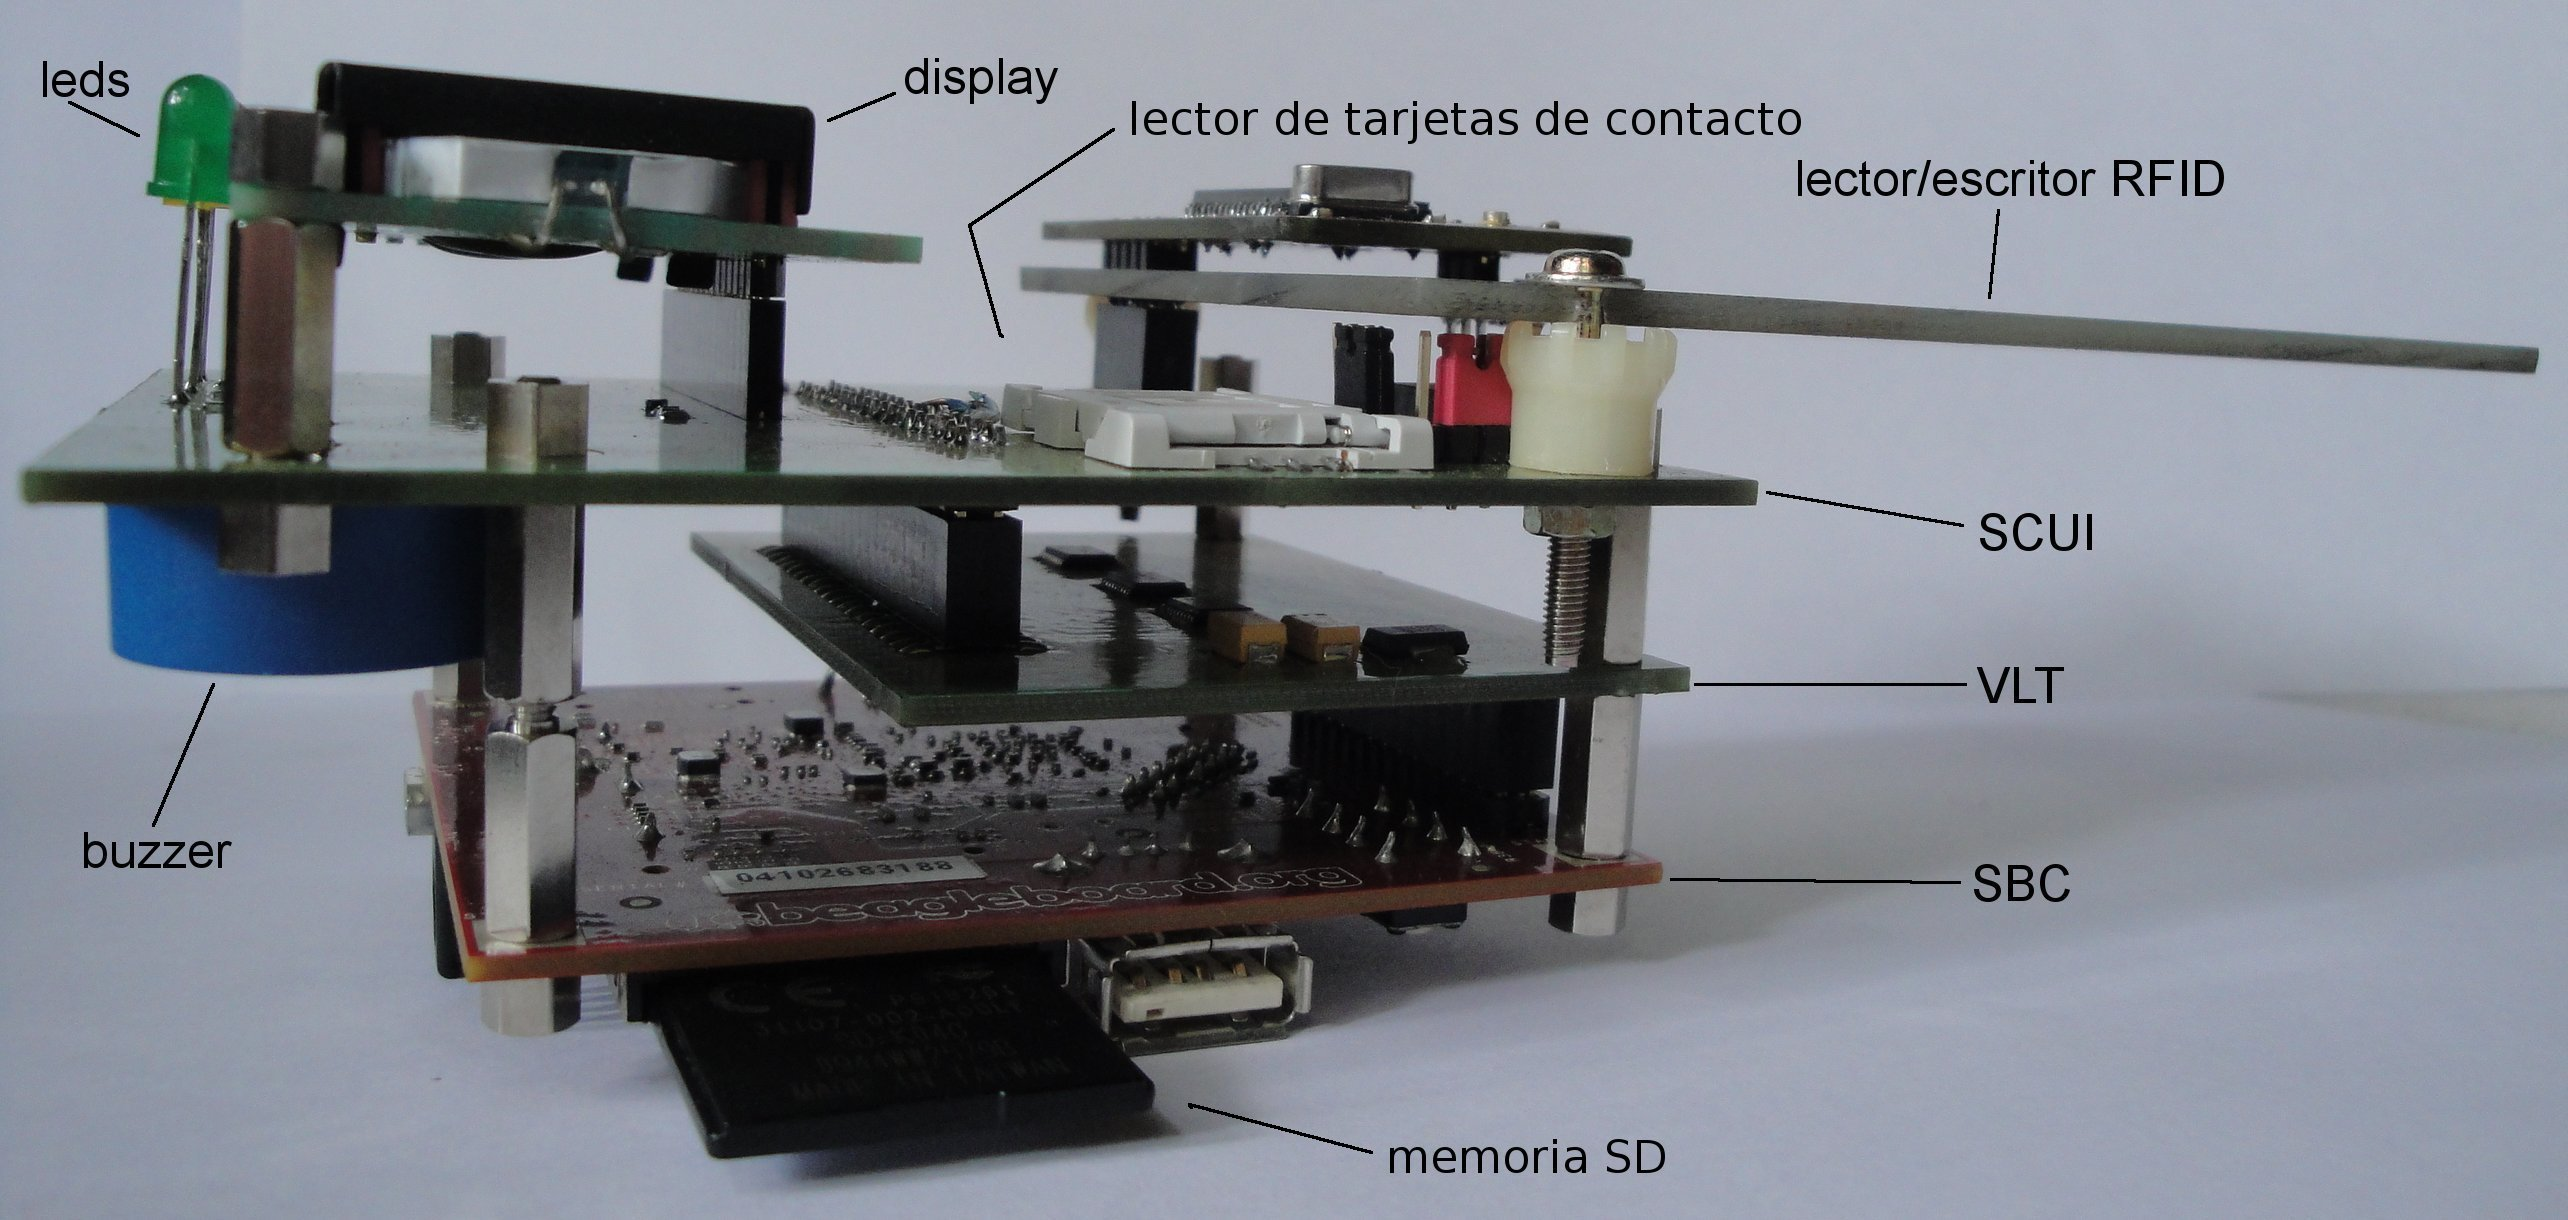
\includegraphics[scale=.12]{Imagenes/prototipo_s_nombres.jpg}
	\end{center}
\end{frame}

\begin{frame}
	\frametitle{SBC}
	Beagleboard:
	\begin{figure}
		\centering		
  		\subfigure{
	  		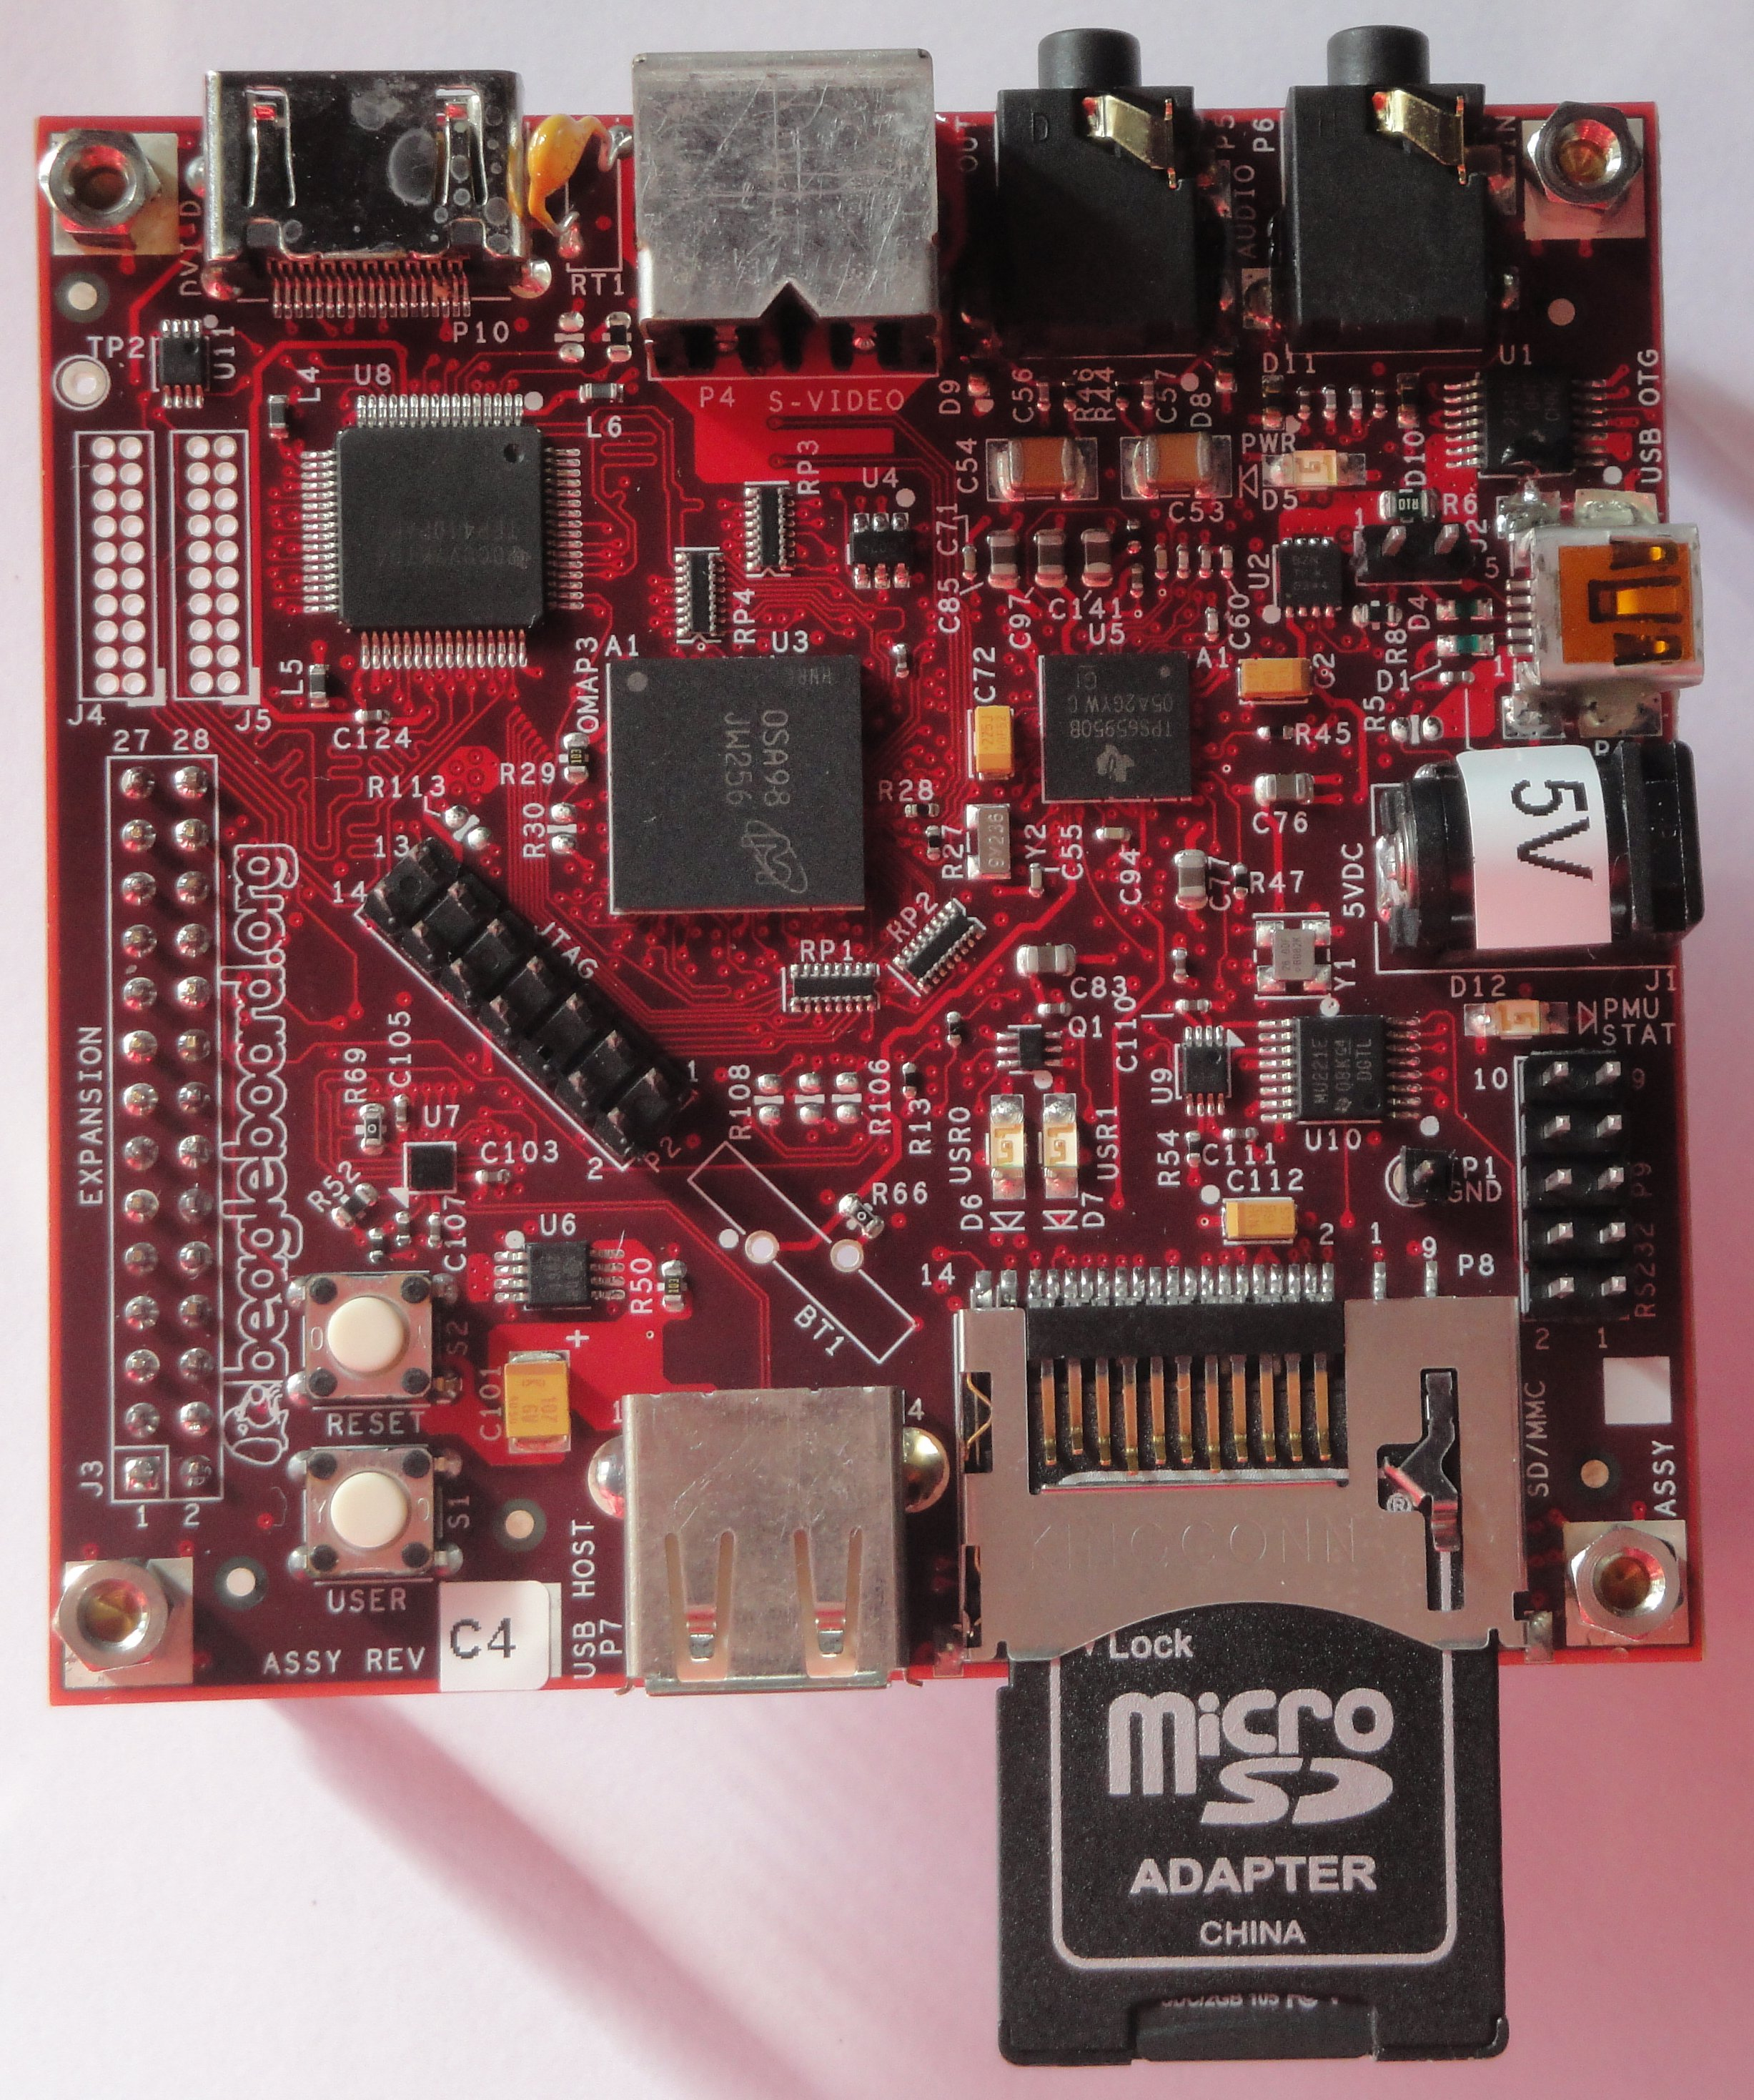
\includegraphics[scale=.03]{Imagenes/SBC_f.jpg} } 
	  	\subfigure{
	  		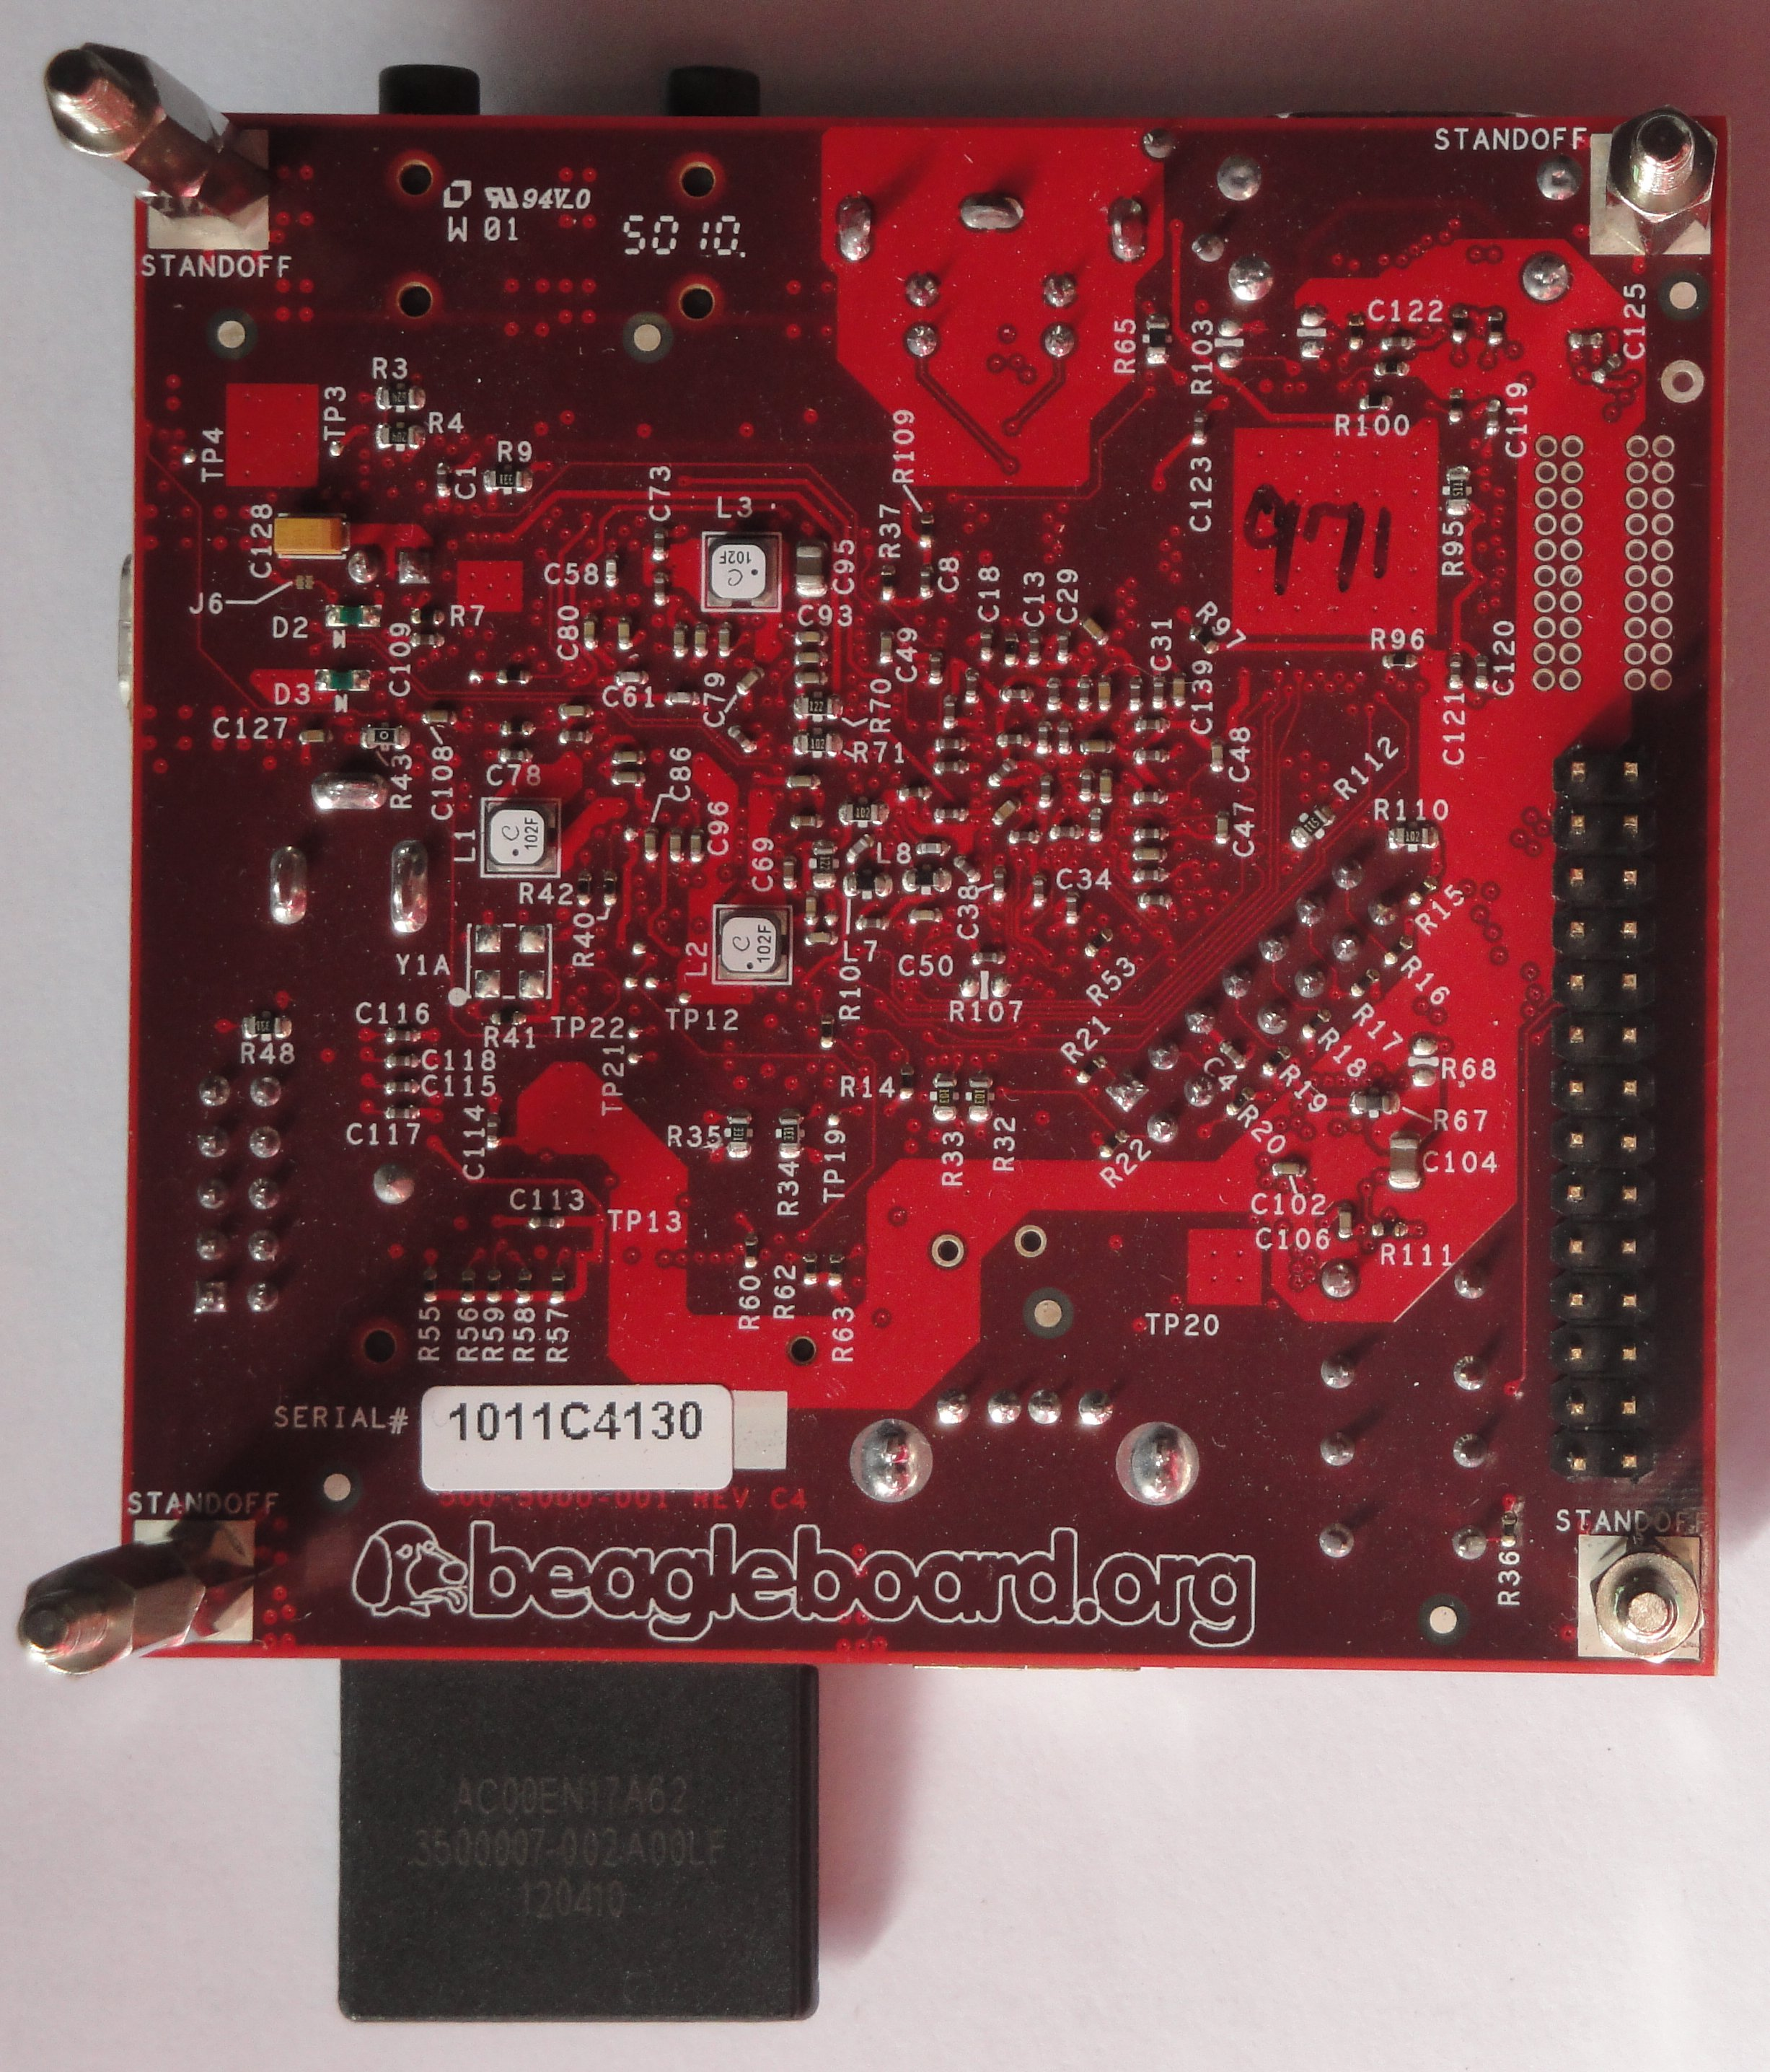
\includegraphics[scale=.03]{Imagenes/SBC_b.jpg} }
	\end{figure}

\begin{itemize}
\item es el sistema basado en un microprocesador
\item se compró
\item ejecuta el sistema operativo
\end{itemize}
\end{frame}

\begin{frame}
	\frametitle{SCUI}
	Lector de tarjetas de contacto e interfaz de usuario:
	\begin{figure}
		\subfigure{
  			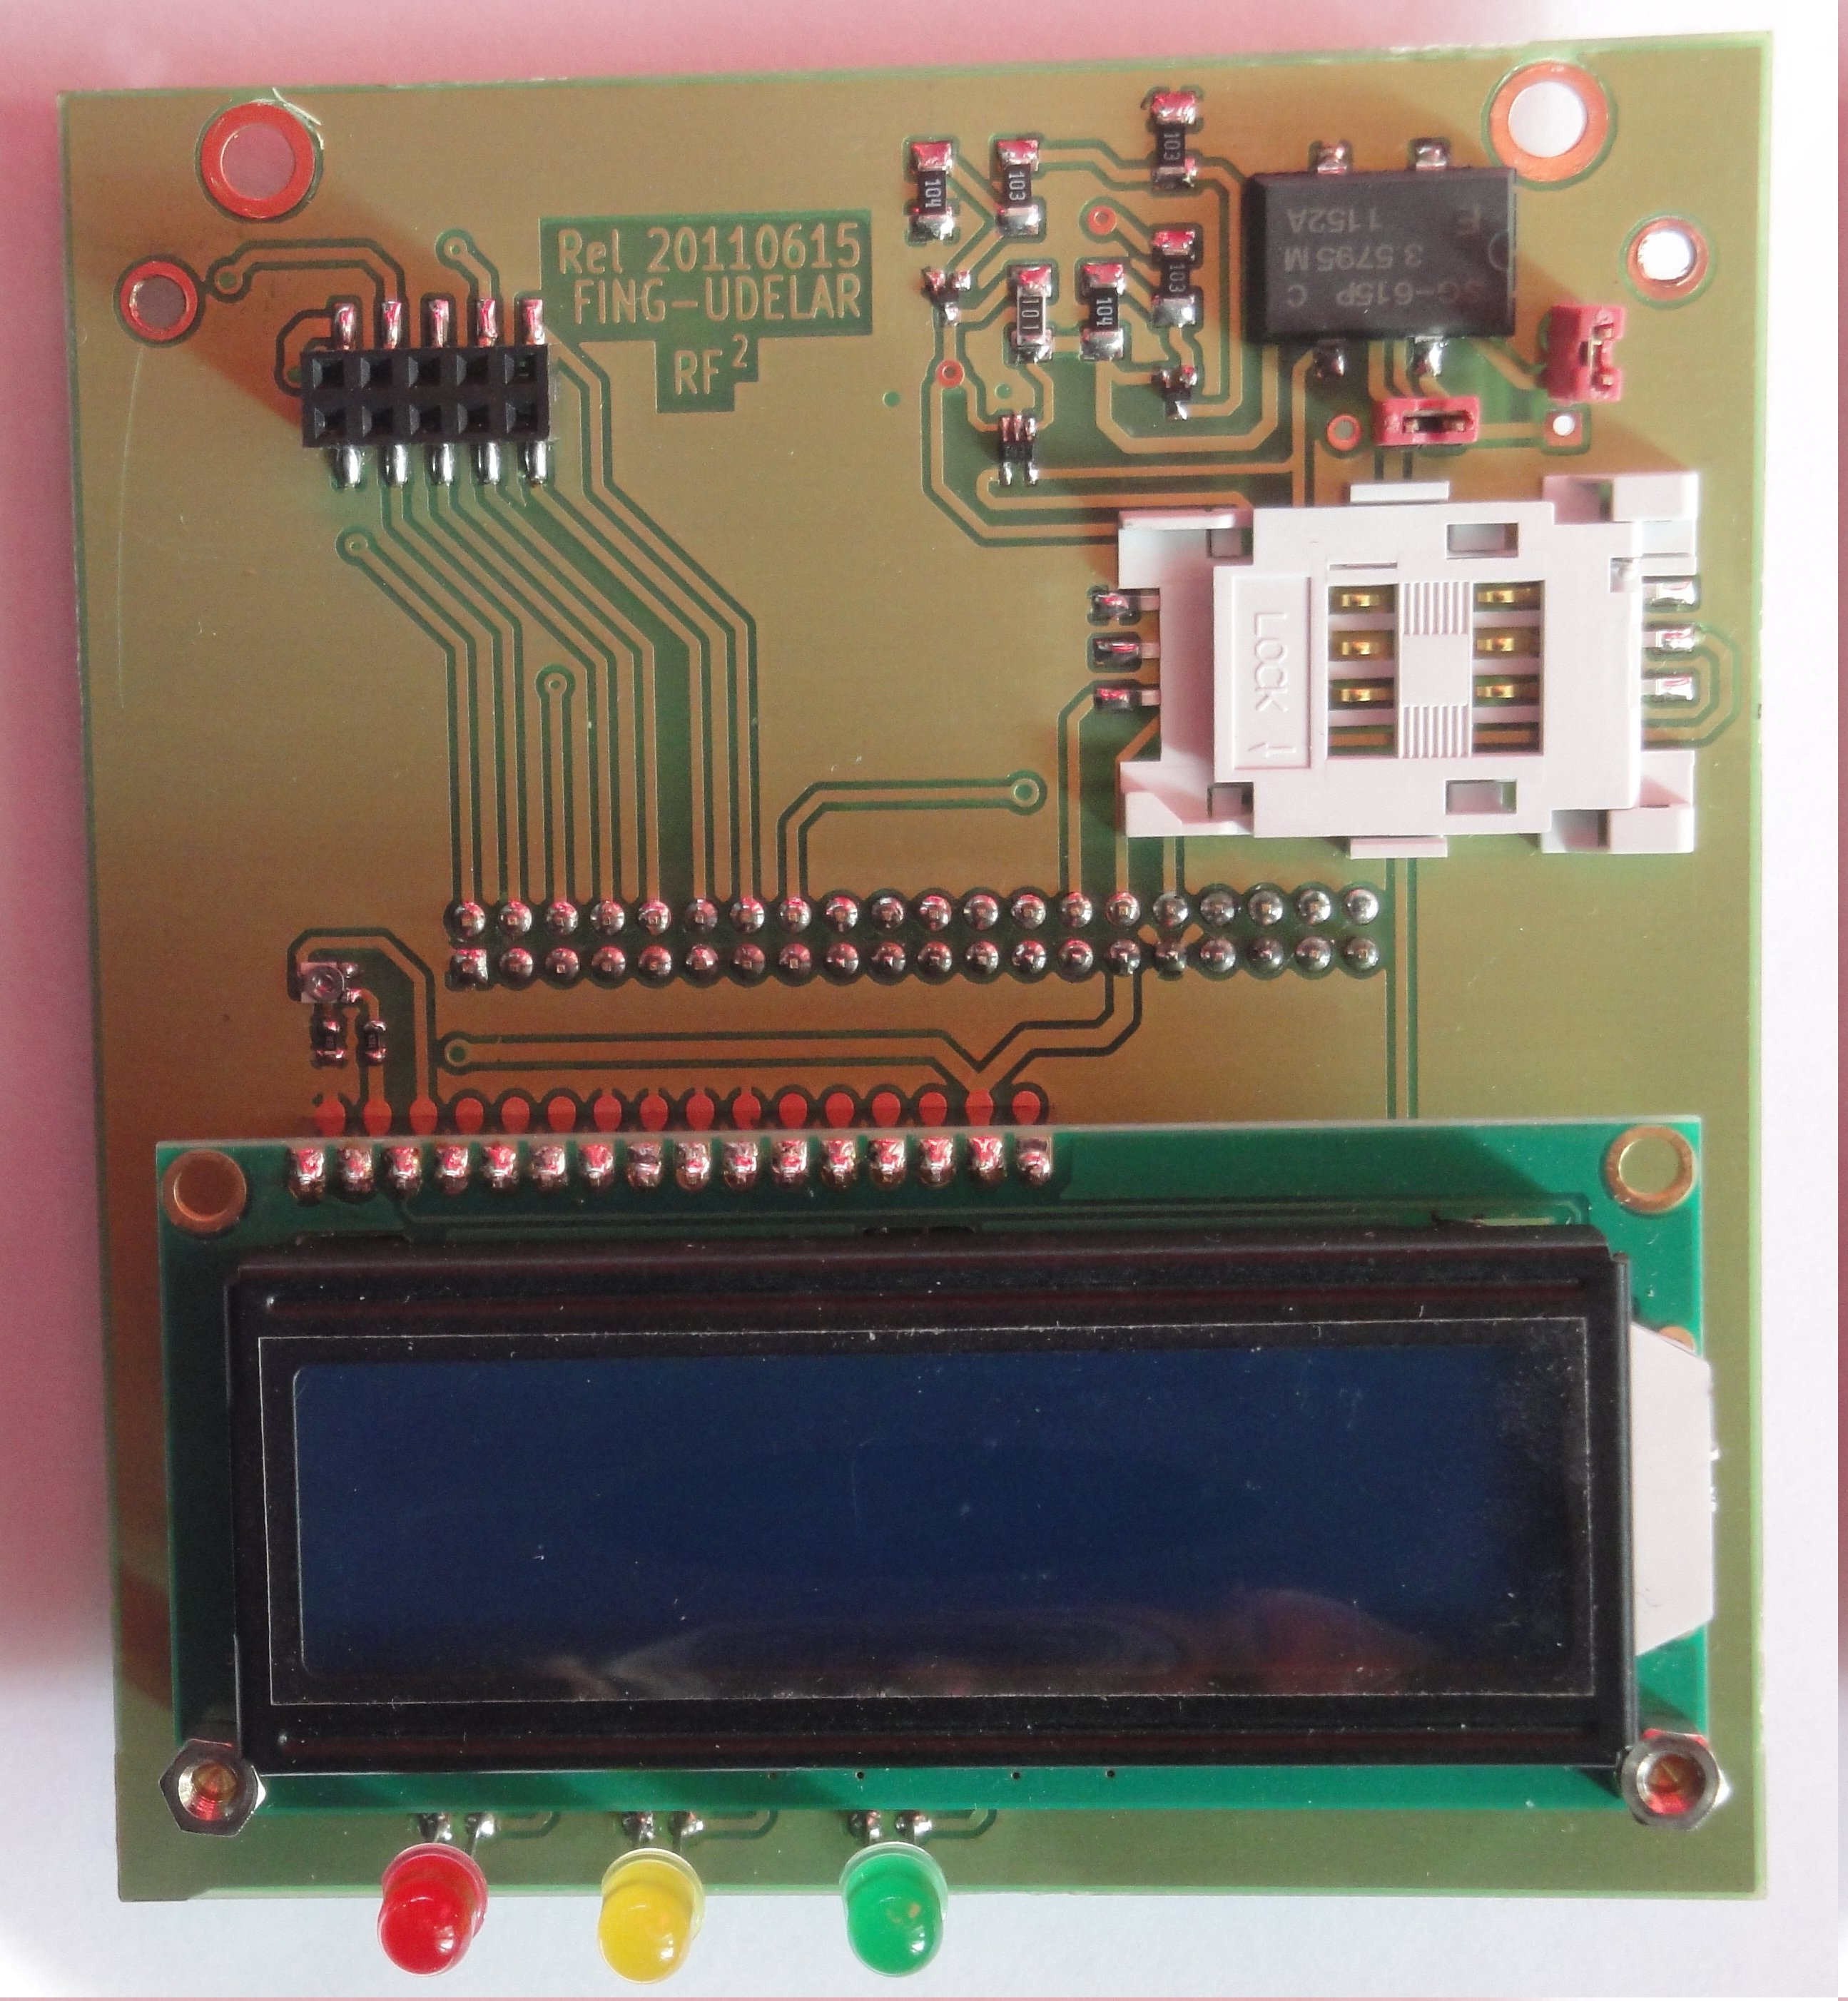
\includegraphics[scale=.03]{Imagenes/SCUI_f.jpg} } 
		\subfigure{ 
			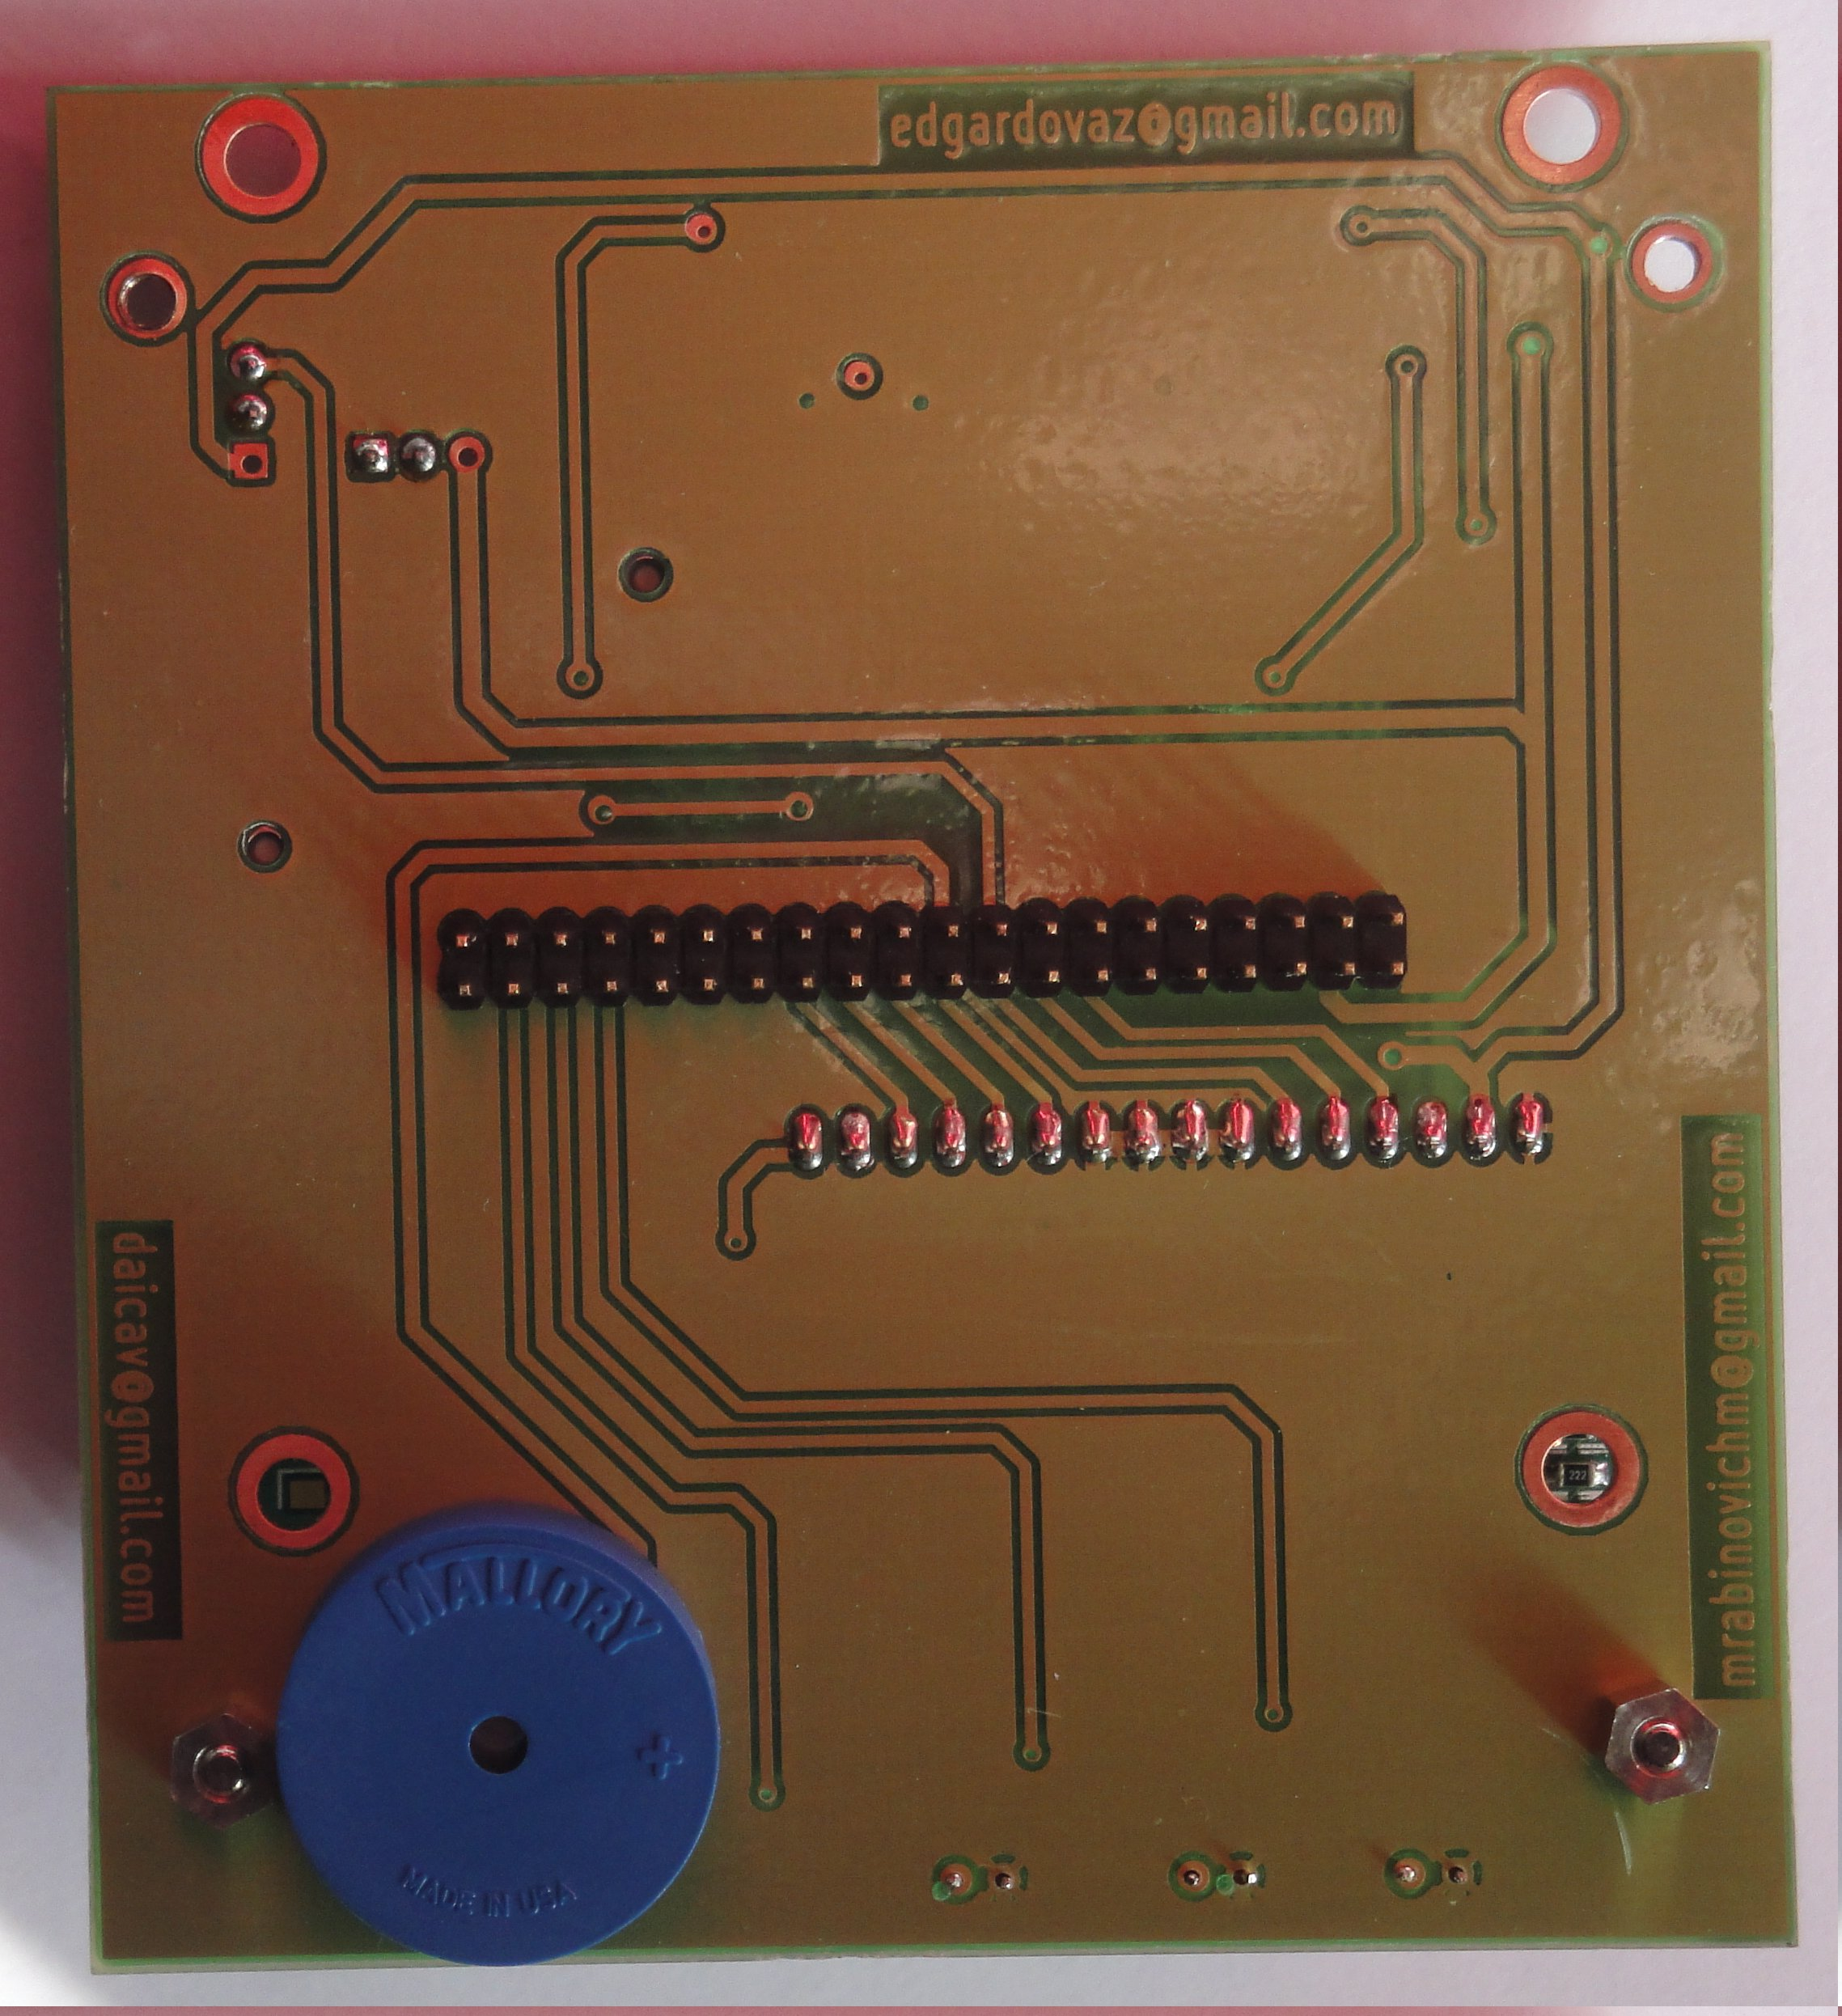
\includegraphics[scale=.033]{Imagenes/SCUI_b.jpg} }
	\end{figure}

\begin{itemize}
\item se integran en un mismo PCB
\item no contiene ASICs
\item se diseñó y fabricó completamente
\end{itemize}
\end{frame}

\begin{frame}
	\frametitle{RFID}
	Lector/escritor de tarjetas RFID:
	\begin{figure}
		\subfigure{
  			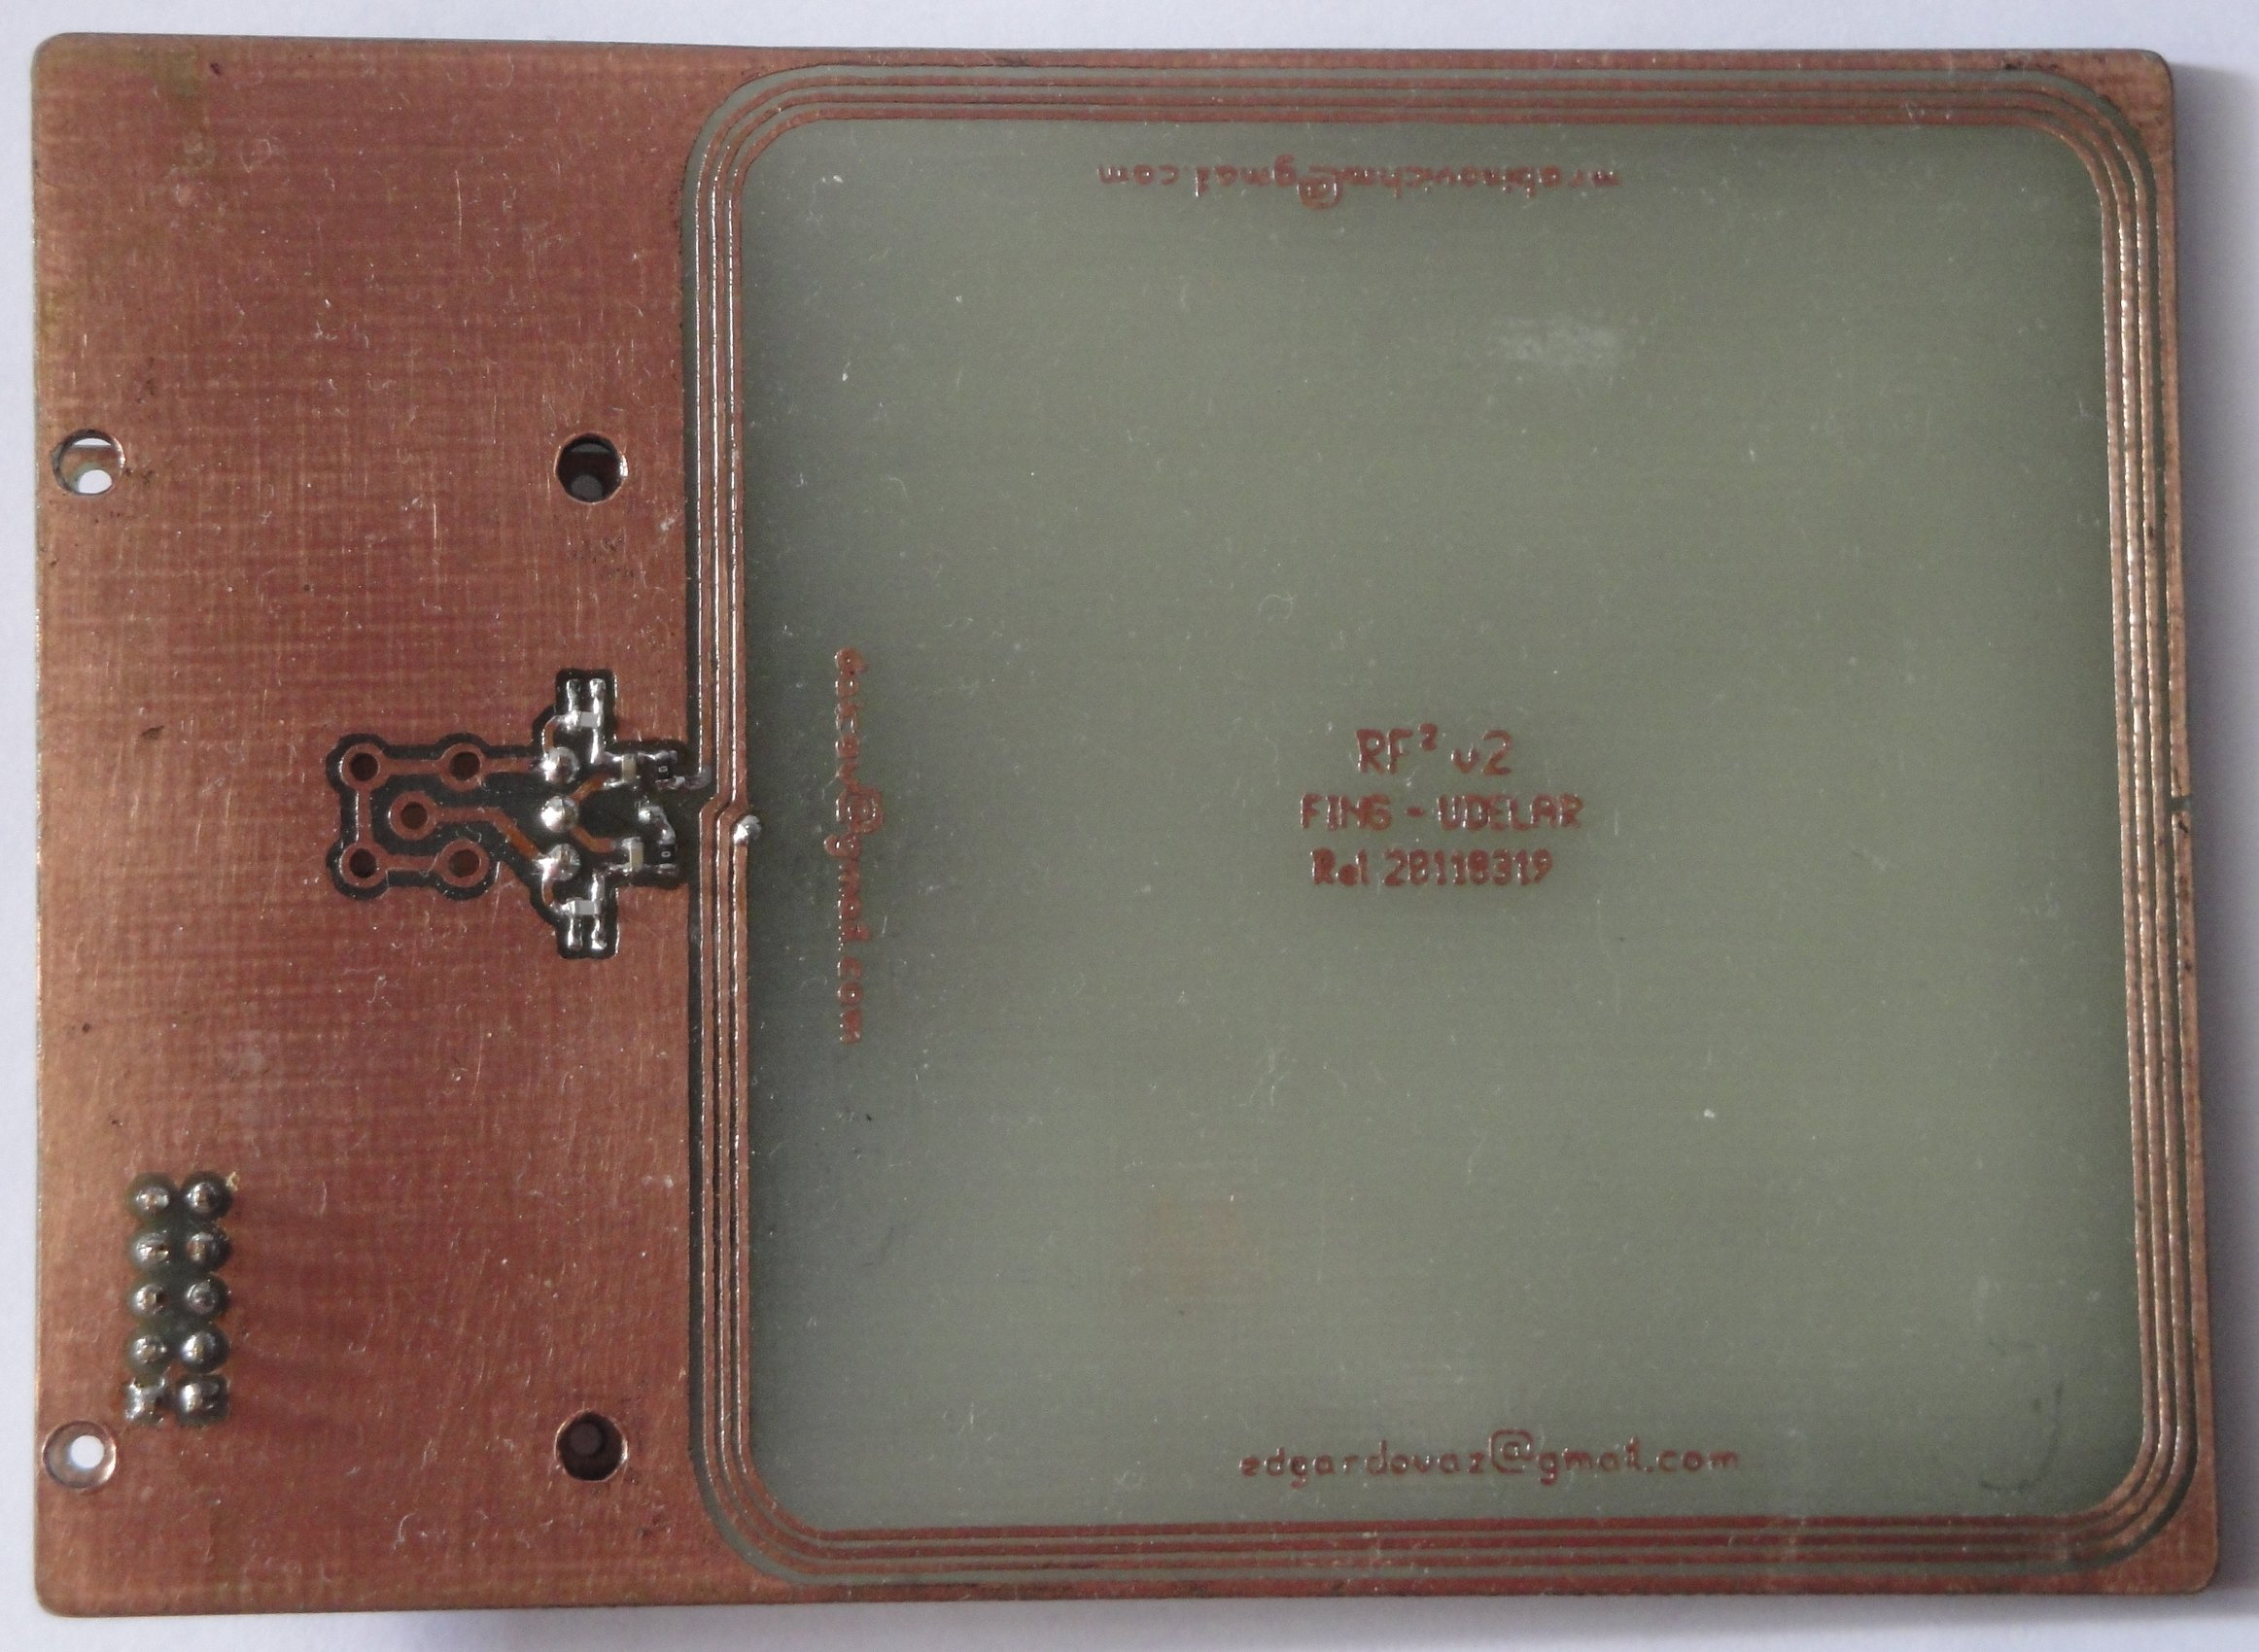
\includegraphics[scale=.04]{Imagenes/ant_f.jpg} } 
		\subfigure{ 
			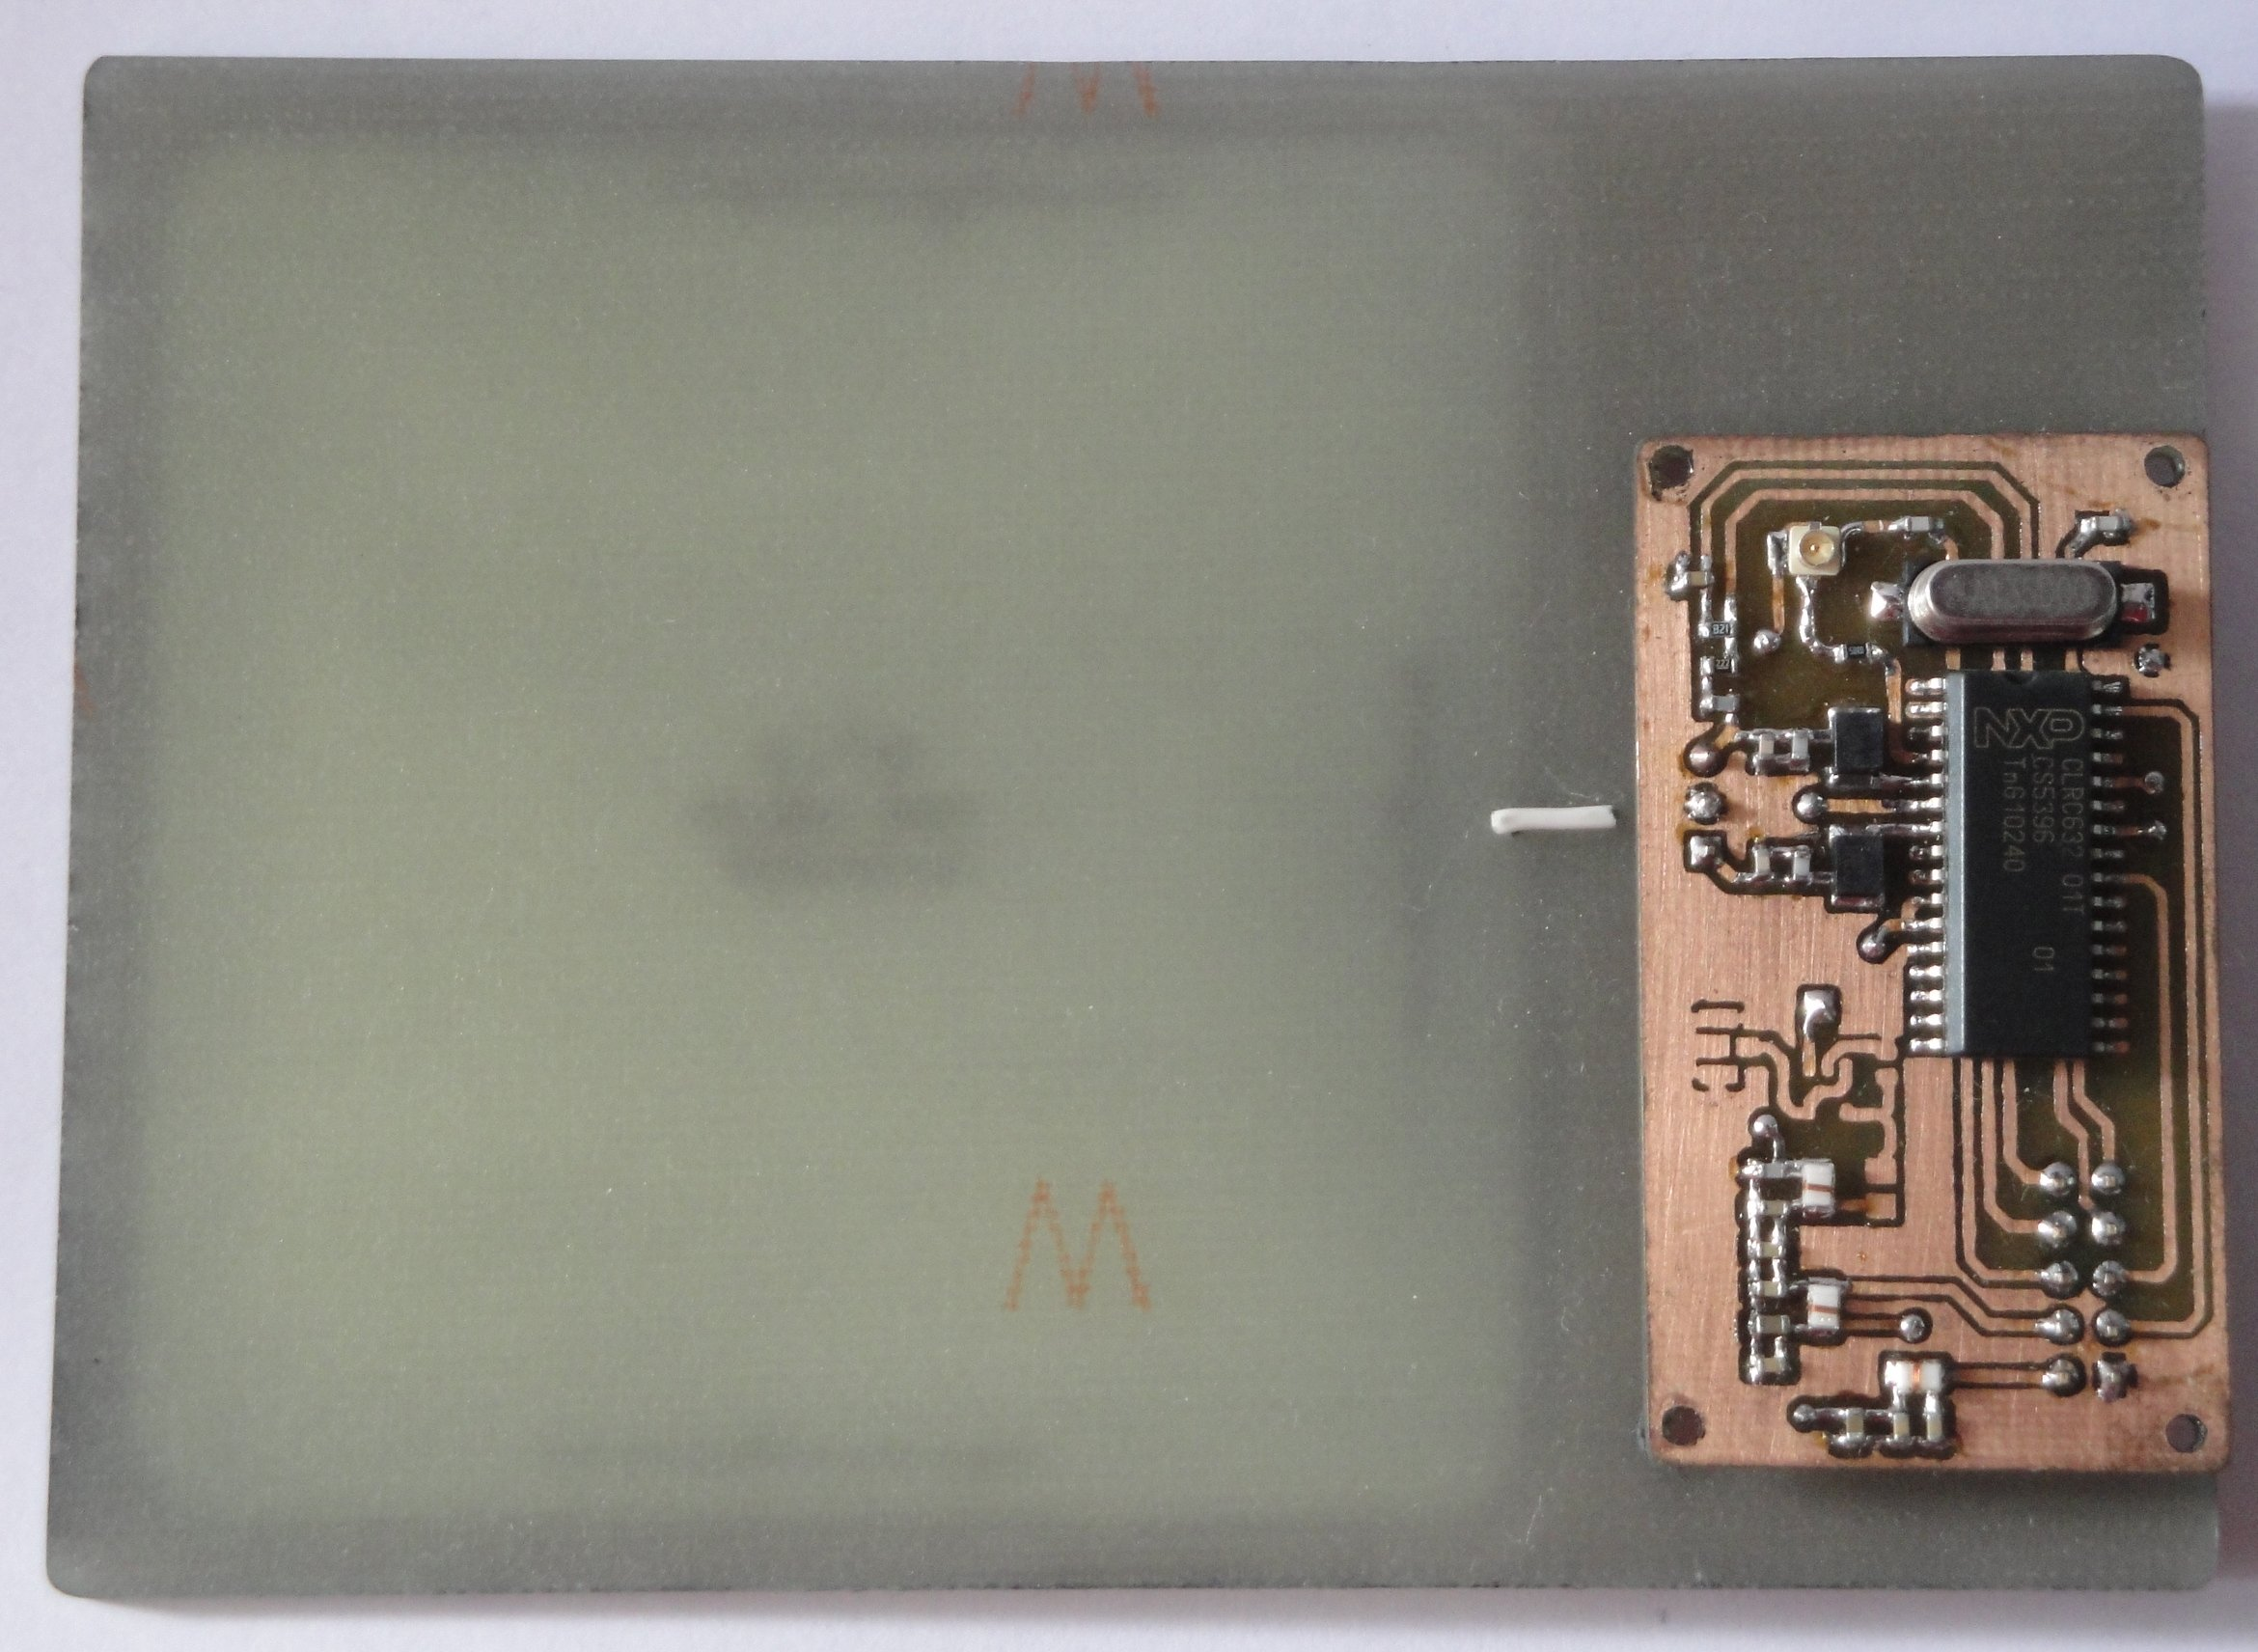
\includegraphics[scale=.04]{Imagenes/ant_b.jpg} }
	\end{figure}

\begin{itemize}
\item PCB a 2 capas
\item tarjetas sin contacto (13,56MHz)
\item CL RC632 se encarga del protocolo para las tarjetas (Mifare)
\item se diseñó y fabricó completamente
\end{itemize}
\end{frame}

\begin{frame}
	\frametitle{Descripción general de funcionamiento}
	\textcolor{red}{acá va el diagrama con las partes? (i+12 de lo planeado)}
\end{frame}	
	
\section{Software}
\subsection{Diagrama de flujo simplificado}
\begin{frame}
	\frametitle{Diagrama de flujo simplificado}
	\textcolor{red}{acá va el diagrama de flujo :)}
\end{frame}		
	
\subsection{Software empleado}
\begin{frame}
	\frametitle{Software}
	\begin{itemize}
		\item Sistema Operativo GNU/Linux
		\item Distribución Angström
		\item Herramientas de desarrollo: 
		\begin{itemize} 
			\item OpenEmbedded-Bitbake 
			\item Narcissus 
		\end{itemize}
	\end{itemize}
\end{frame}		

\subsection{Bibliotecas}
\begin{frame}
	\frametitle{Bibliotecas}
	\begin{itemize}
		\item librfid, editada (herramienta librfid-tool contiene el programa principal)
		\item libgpio, completamente implementada
		\item liblcd, editada (completamente implementada en 2009)
		\item libpcsclite
	\end{itemize}

\textcolor{red}{diagrama de capas de software}
\end{frame}

\begin{frame}
	\frametitle{Bibliotecas}
	\textcolor{red}{diagrama de capas de software librfid-tool}

	Funciones de utilidad de la herramienta librfid-tool:
	\begin{itemize}
		\item lectura de tarjeta completa
		\item lectura de un sector específico
		\item escritura de un sector específico
	\end{itemize}
\end{frame}

\section{Ensayos}

%\subsection{Campos de aplicación}
%\begin{frame}
%	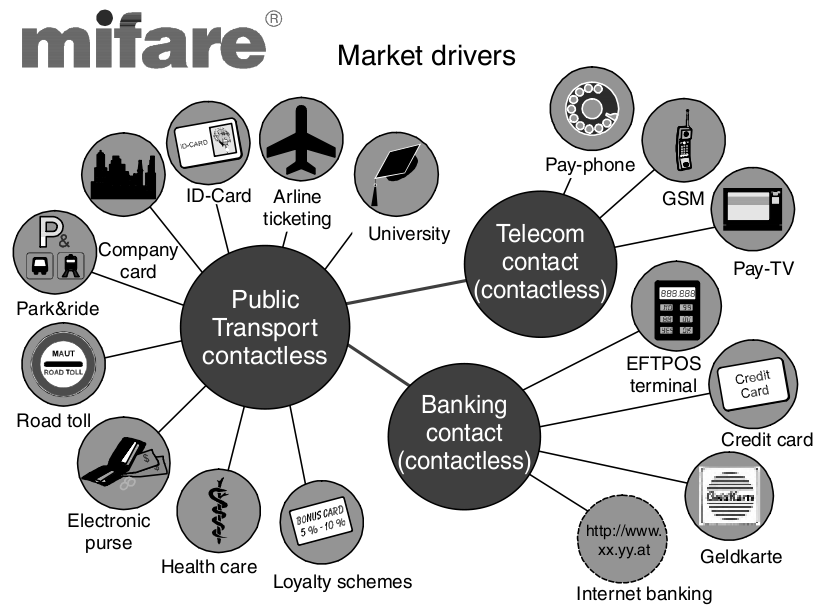
\includegraphics[scale=.4]{Imagenes/aplicaciones.png}
%\end{frame}


%%%%%%%%%%%

\section{Preguntas}
\begin{frame}
	\begin{center}
		\bigskip		
		
\includegraphics[scale=.5]{Imagenes/preg.jpg}
	\end{center}
\end{frame}

\end{document} 